\section{Experimental work}

\subsection{Setup}
The hardware setup that hosts the training and testing experiments is a personal computer with Intel Core i7-9750H CPU, Nvidia GeForce RTX 2060 GPU, and 16GB of RAM. Unity real-time 3D Game Engine\cite{Unity} is the simulator adopted for creating the training environment and evaluating the proposed platoon structure with the help of the developed ML-Agents toolkit\cite{juliani2018unity} within Unity that enables the integration between Unity Editor and training the multi-agent cooperative platoon.

\subsection{Training}
A platoon of only three vehicles is trained using Proximal Policy Optimization (PPO) based on end-to-end deep reinforcement learning to learn a robust cooperative driving behavior. PPO has shown better results over other RL algorithms while being more empirical for having better sample complexity \cite{juliani2018unity},\cite{schulman2017proximal}, \cite{ye2020automated}. Most of the PPO hyperparameters are set to the default values supported by the ML-Agents toolkit or adopted from other studies' recommendations as in \cite{gupta2021embodied}. Deep Neural Network consists of 5 layers of shape \{35,256,256,256,2\}. Figure 7 visualizes the Network, the input layer that takes ego perception, the gap between follower and predecessor vehicles, and shared predecessor perception. Then 3 fully connected hidden layers with 256 neurons each, and the output layer consists of two neurons which are the steering and throttle of each vehicle. All vehicles in the platoon have the same trained model with the same neural network layer, except for the leader vehicle the V2V perception data input is off.

\begin{figure}[H]
    \centering
    %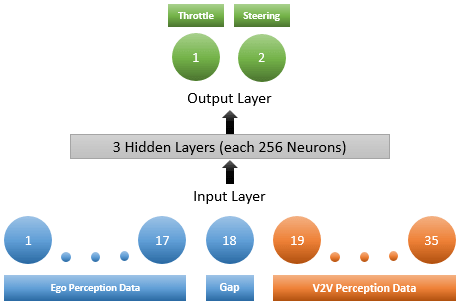
\includegraphics[scale=0.5]{Figures/NNetwork6-min.PNG}
    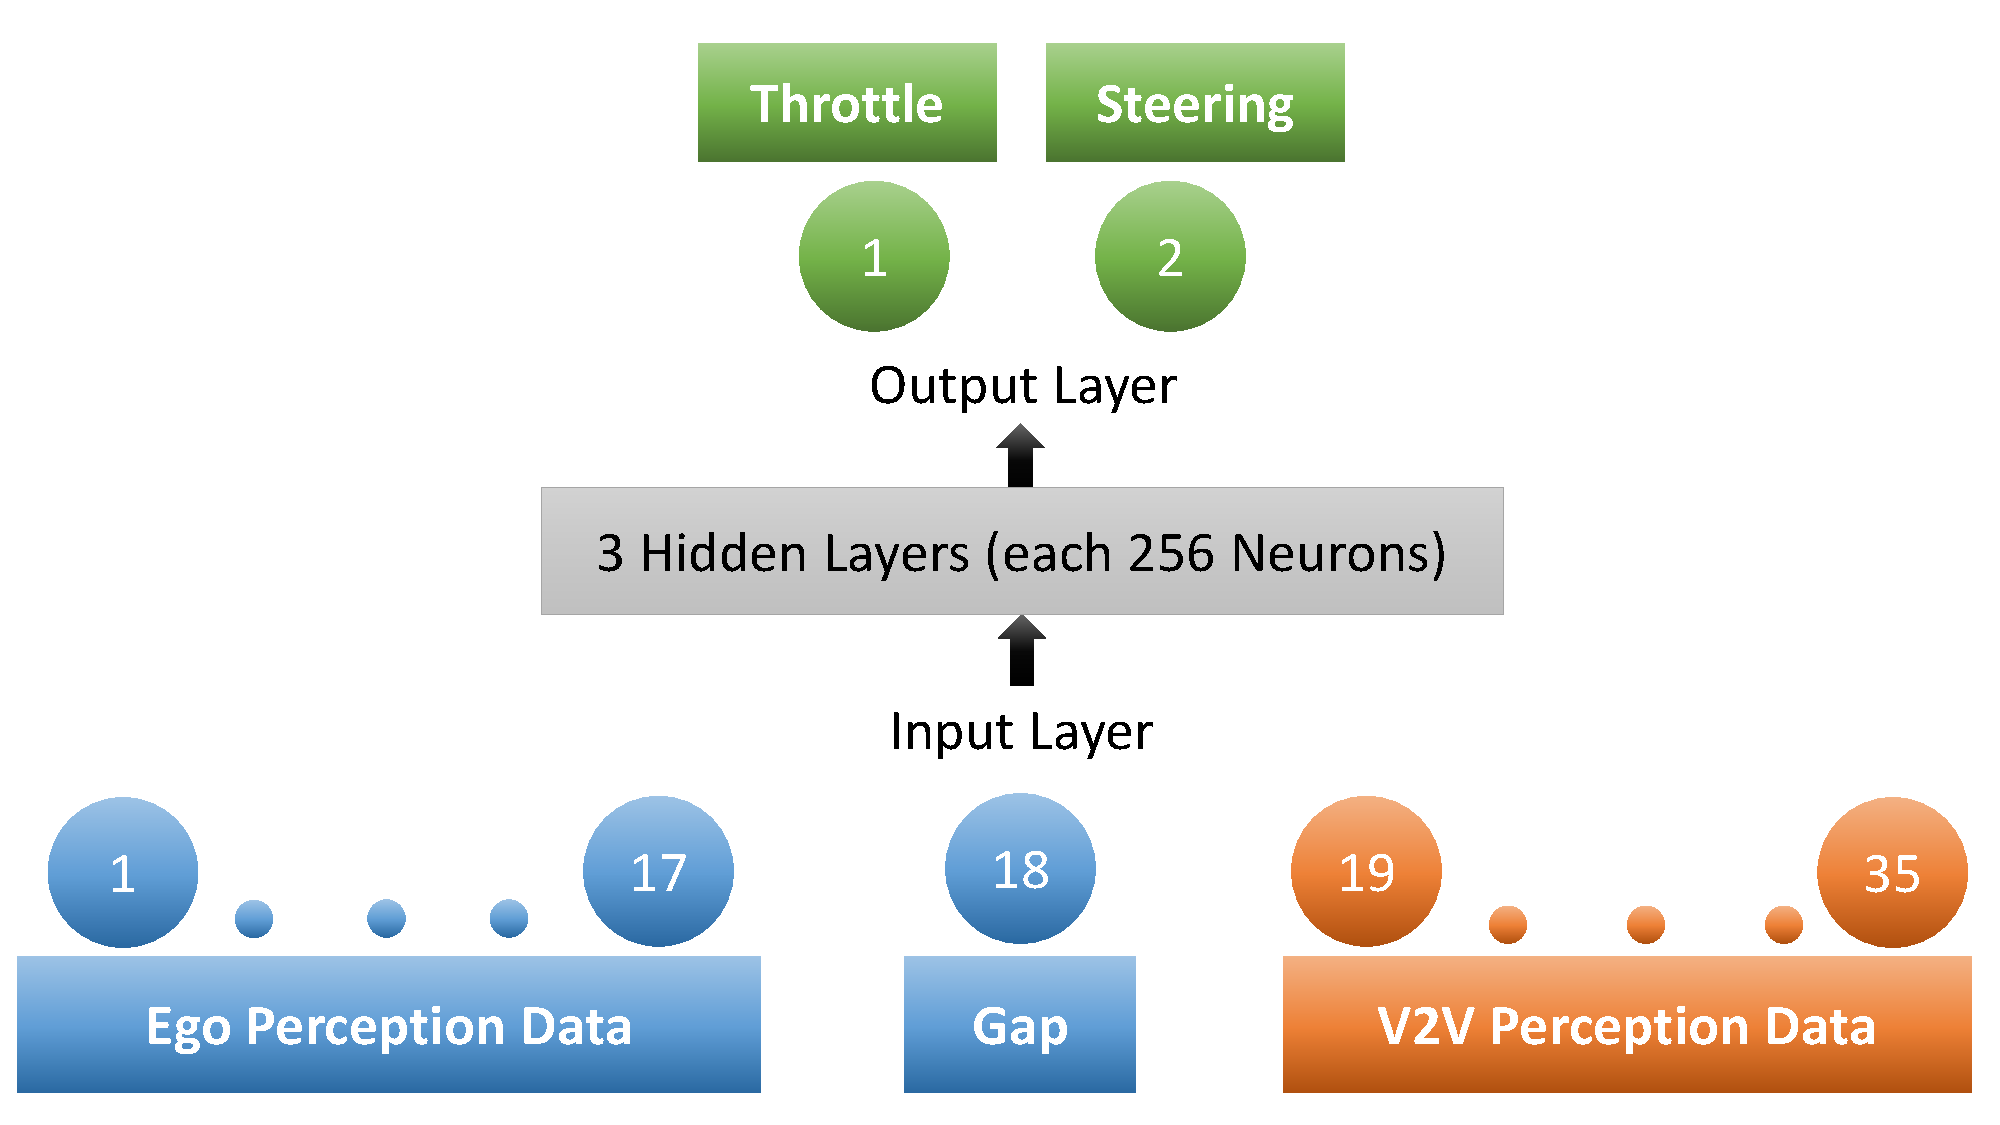
\includegraphics[width=0.7\linewidth]{Figures/NN_compressed.pdf}
    \caption{Deep Neural Network Layers}
    \label{fig:my_label}
\end{figure}

\begin{comment}
\begin{figure}[H]
    \centering
    %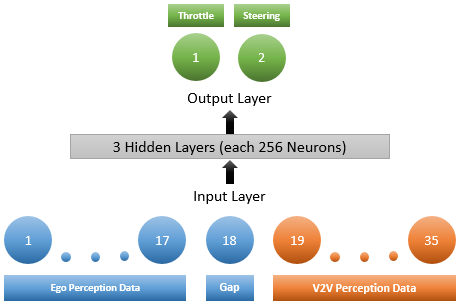
\includegraphics[scale=0.35]{Figures/NNetwork6.PNG}
    %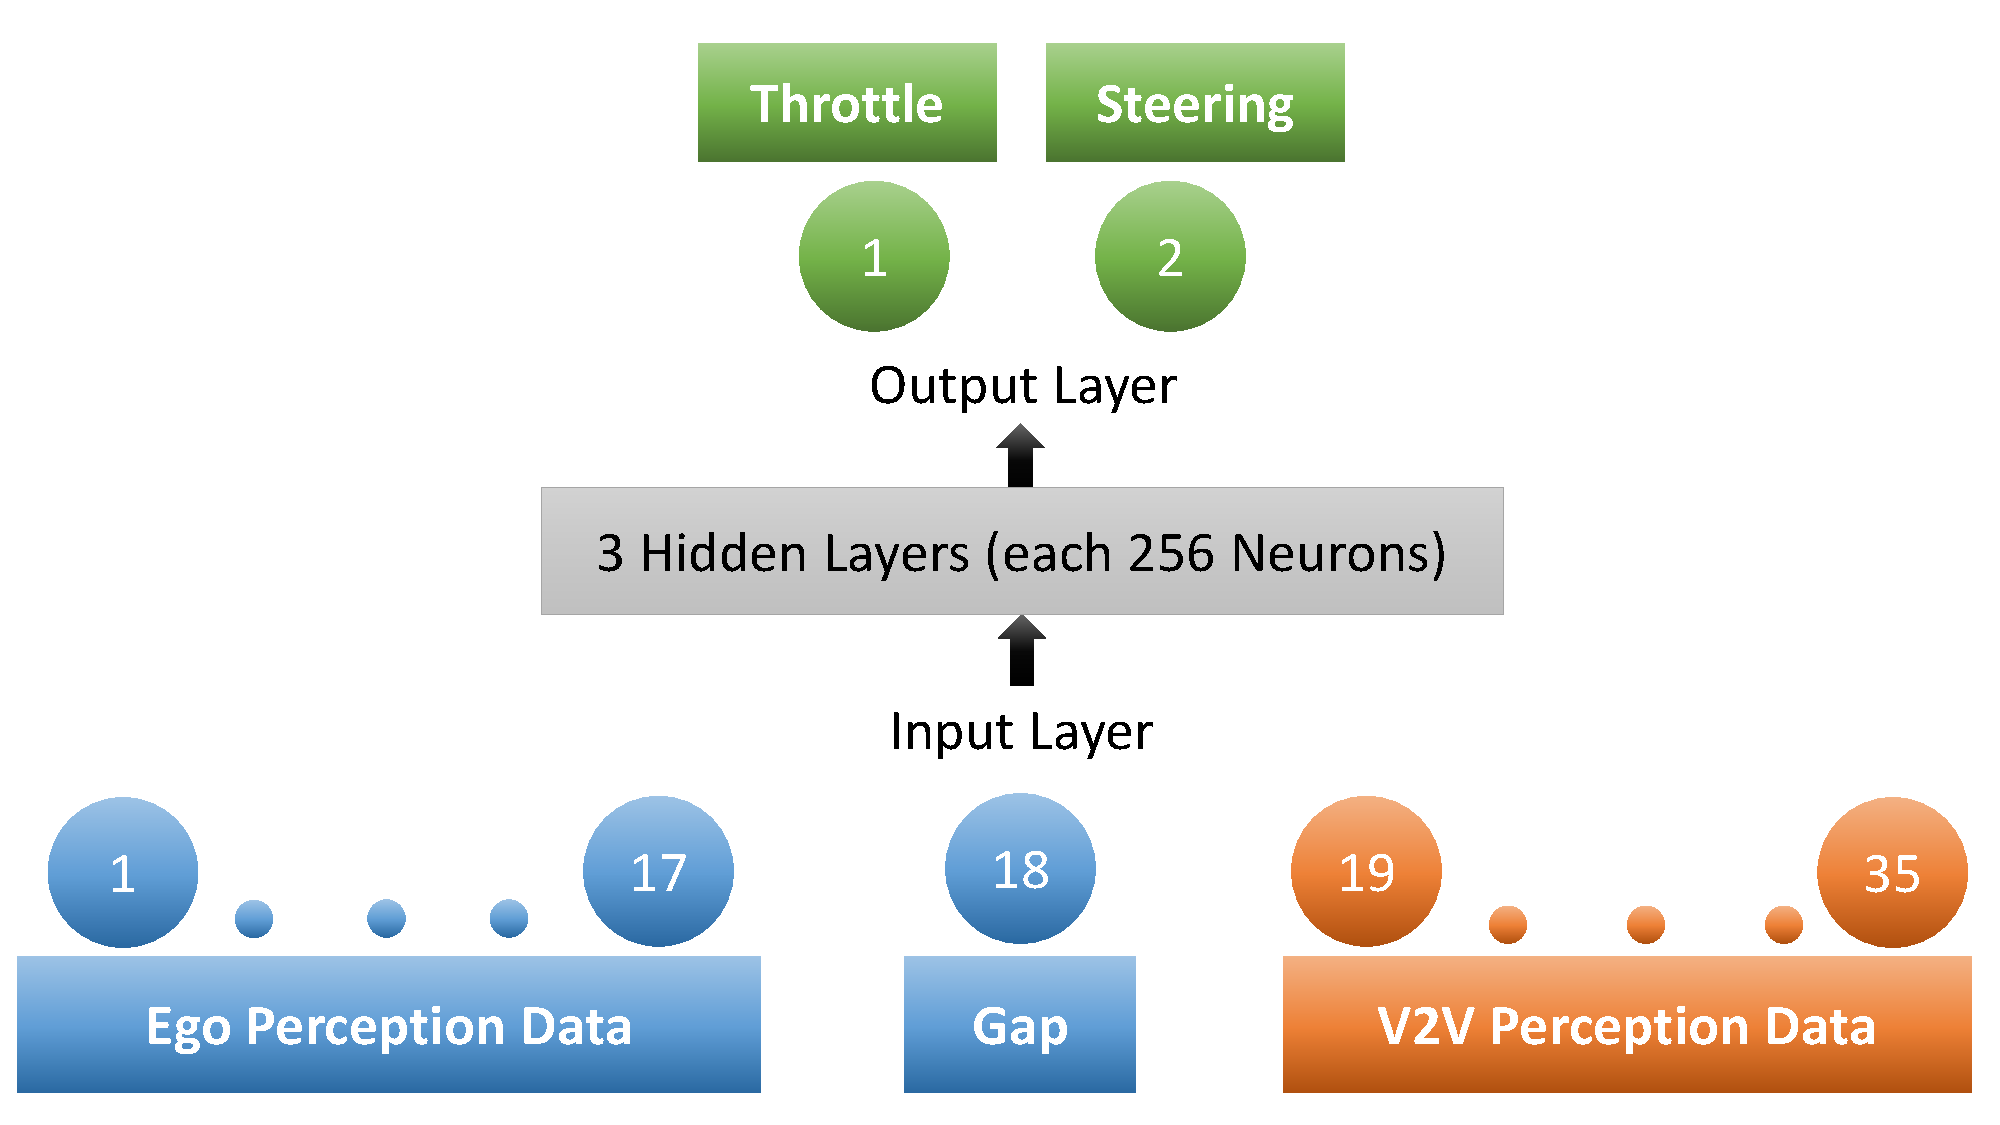
\includegraphics[scale=0.35]{Figures/NN.pdf}
    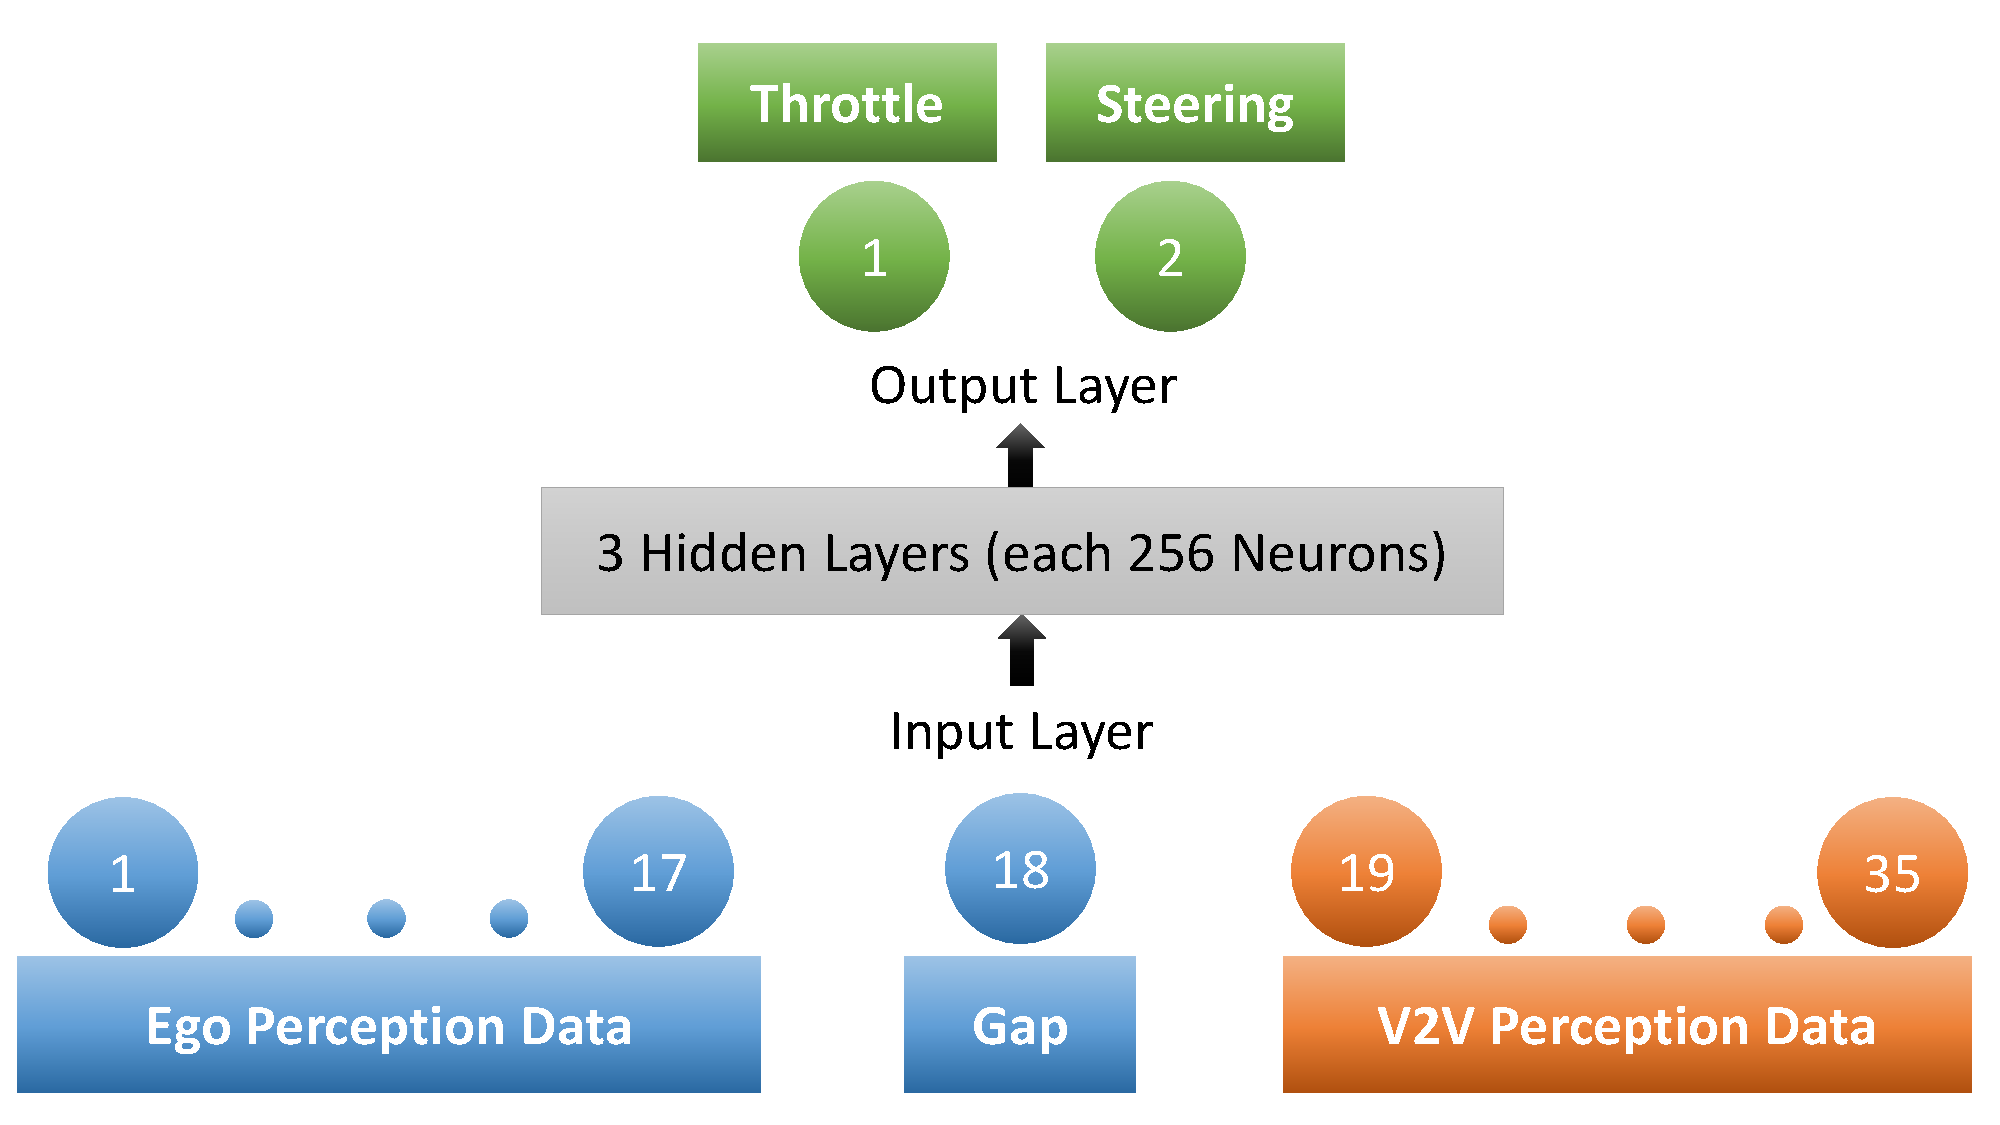
\includegraphics[width=0.6\linewidth]{Figures/NN.pdf}
    \caption{Deep Neural Network Layers}
    \label{fig:my_label}
\end{figure}
\end{comment}




Figure 8, shows the training track with a total driving distance of 1300 meters. Vehicles are trained to drive safely in a cooperative system (platoon). while caring about their rewards and other vehicles' rewards like avoiding penalties for crashing. Training is applied on two parallel environments with the same track design but the positions of obstacles are changed to avoid model over-fitting and parallel environments decrease the training time.
\begin{figure}
    \centering
    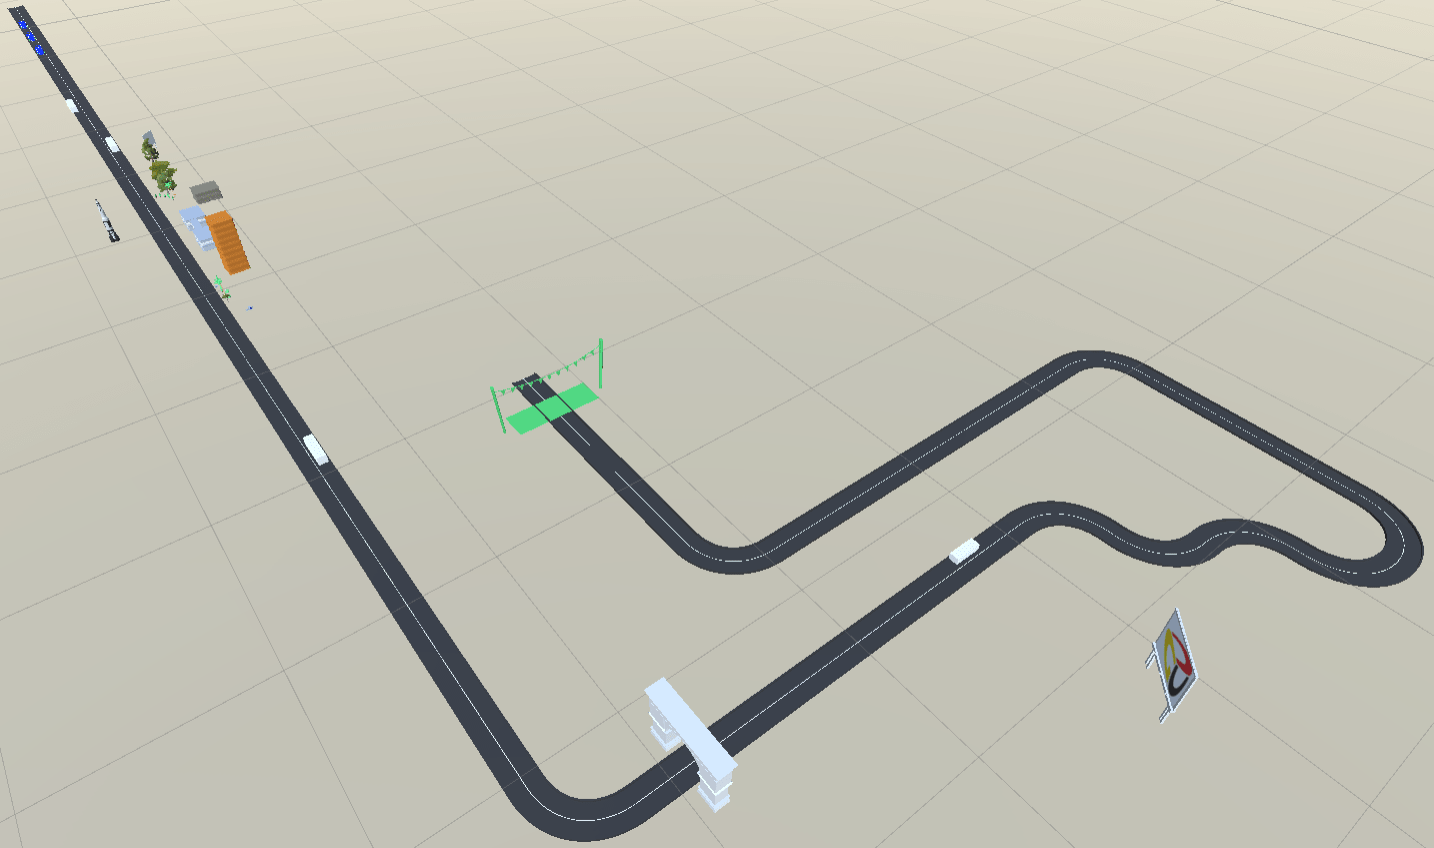
\includegraphics[width=9cm,height=5cm,keepaspectratio]{Figures/EnvTraining6-min.PNG}
    %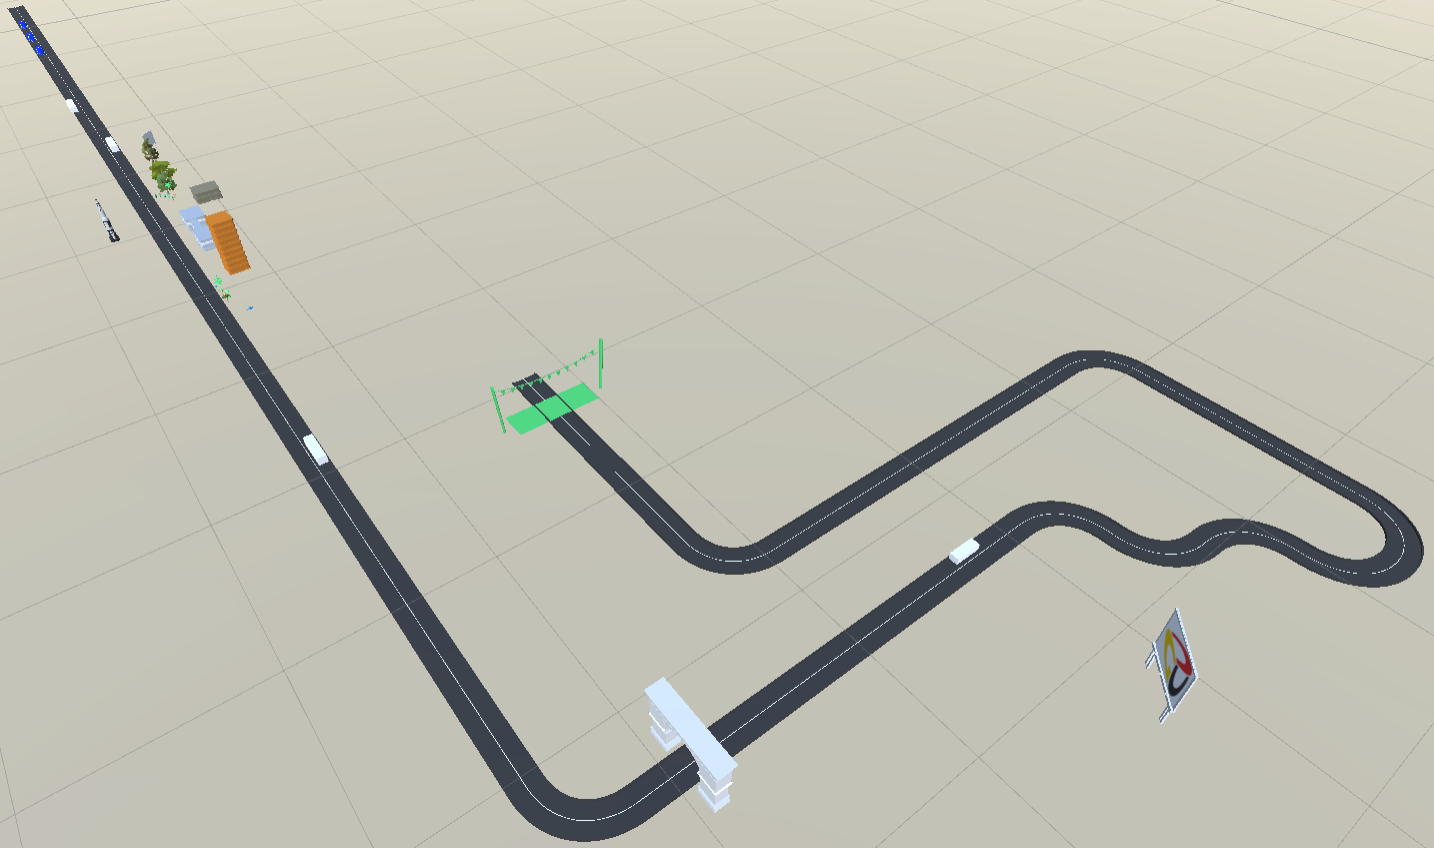
\includegraphics[scale=0.3]{Figures/EnvTraining6.PNG}
    \caption{Urban Training Track}
    \label{fig:my_label}
\end{figure}









\begin{comment}
\begin{figure}[H]
    \centering
    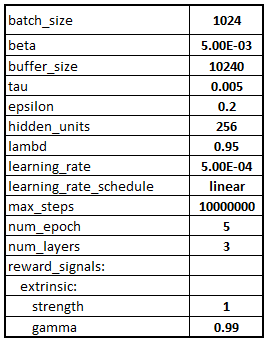
\includegraphics[scale=0.4]{Figures/PPOHyp.PNG}
    \caption{MDP}
    \label{fig:my_label}
\end{figure}

\begin{table}[H]
\centering
\caption{PPO hyperparameters} 
\resizebox{8.5cm}{!}{
\begin{tabular} {|c||c|c|c|} 
 \hline
 Hyperparameter & Value\\
 \hline
 Discount $\gamma$ & 0.99\\
\hline
\end{tabular} }
\end{table}
\end{comment}

\begin{comment}
\subsection{RL Reward Signals}
Reward shaping is a very critical aspect in RL training performance as it is the way of communication to the agent to evaluate it in order to achieve the required behavior.
Curriculum Learning\cite{bengio2009curriculum} is applied on penalties like those caused by crashes to let vehicles have the courage to train with fewer worries about negative rewards at the beginning of training and then penalties' values are increased to give higher priority to safe driving and avoid any crashes or platoon dissociation. If penalties are high from the start of training, sometimes agents decide to stop driving or are afraid of taking any action that may lead to high negative rewards and this slows down the training progress and may lead to passive, not active behavior.

All vehicles in the platoon are subjected to the same positive rewards as shown in Table I, which are the reward signals that focus on teaching vehicles that they should drive on the right lane and as fast as possible to collect more positive rewards. Penalties or negative rewards are the reward signals that teach vehicles safe driving (avoid crashing with track borders, obstacles, or other vehicles). These numerical values for reward signals are subjected based on suggestions from ML-Agents toolkit documentation, and trial and error method.
Table I presents rewards for only the discrete events, while speed and gap error penalties are subjected on each time step.

\begin{table}[H]
\centering
\caption{Reward Signals for Discrete Events} 
\resizebox{8.5cm}{!}{
\begin{tabular} {|c||c|c|c|} 
 \hline
 \textbf{Event} & \textbf{Reward [0-10m]} & \textbf{Reward [10-15m]} & \textbf{Reward [15-25m]}\\
 \hline
 Checkpoints of right lane & 1 & 1 & 1\\
 \hline
 Checkpoints of left lane & -0.1 & -1 & -2\\
\hline
Reach finish line & 100 & 100 & 100\\
\hline
Crash & -10 & -10 & -50\\
\hline
\end{tabular} }
\end{table}

To apply caring between agents, agents should learn that working cooperatively results in positive rewards, and not helping each other results in negative rewards. Each follower vehicle in the platoon cares about the predecessor vehicle and this is applied by giving a positive reward to the predecessor vehicle if the follower reached the finish line and a negative reward in case of crashes. This trains the predecessor vehicle to avoid any aggressive actions that may lead to crashes or disorder behavior among the platoon.

The formulated penalty equation of velocity error for the leader:
\begin{gather}
e_{velocity,l} = V_l - V_{desired} \\
P_{velocity,l} = -(e_{velocity,l}/V_{max})^2
\end{gather}  

Followers are subjected to penalties for gap and velocity errors:

\begin{gather}
e_{velocity,f} = V_f - V_{predecessor} \\
P_{velocity,f} = -(e_{velocity,f}/V_{max})^2\\
e_{gap,f} = G_f - G_{desired}\\
P_{gap,f} = -(e_{gap,f}/G_{max})^2
\end{gather}
where gap between ego vehicle and predecessor vehicle is calculated as follows:
\begin{gather}
G_f = \sqrt{(x_{ego} - x_{pred}) + (z_{ego} - z_{pred})}
\end{gather}

Velocity and gap errors equations are inspired from the work of this study \cite{faragreinforcement} which succeeded in formalizing equations that ease learning for agents in vehicle platooning formation. The vehicle's top speed is 60km/h, the desired gap between vehicles is 10 meters, and the maximum allowable gap between vehicles is 30 meters. The gap error penalty ranges from 0 (10m), to -1 (30m) while if the gap increases to be more than 30m, then the gap penalty is the same as 30m of -1. Rewards on gap and speed errors are applied on each time step of 0.02 seconds. However, other rewards are applied when an event happens like crashing or reaching the finish line.
\end{comment}





\begin{comment}
\subsection{Evaluation metrics}
Evaluating SDCP performance will be criticized by gap error, velocity error, and number of crashes.
The test track is designed to be as complex as training track with new scenario like passing through a narrow way between two static obstacles as shown in figure ?.

\begin{figure}[H]
    \centering
    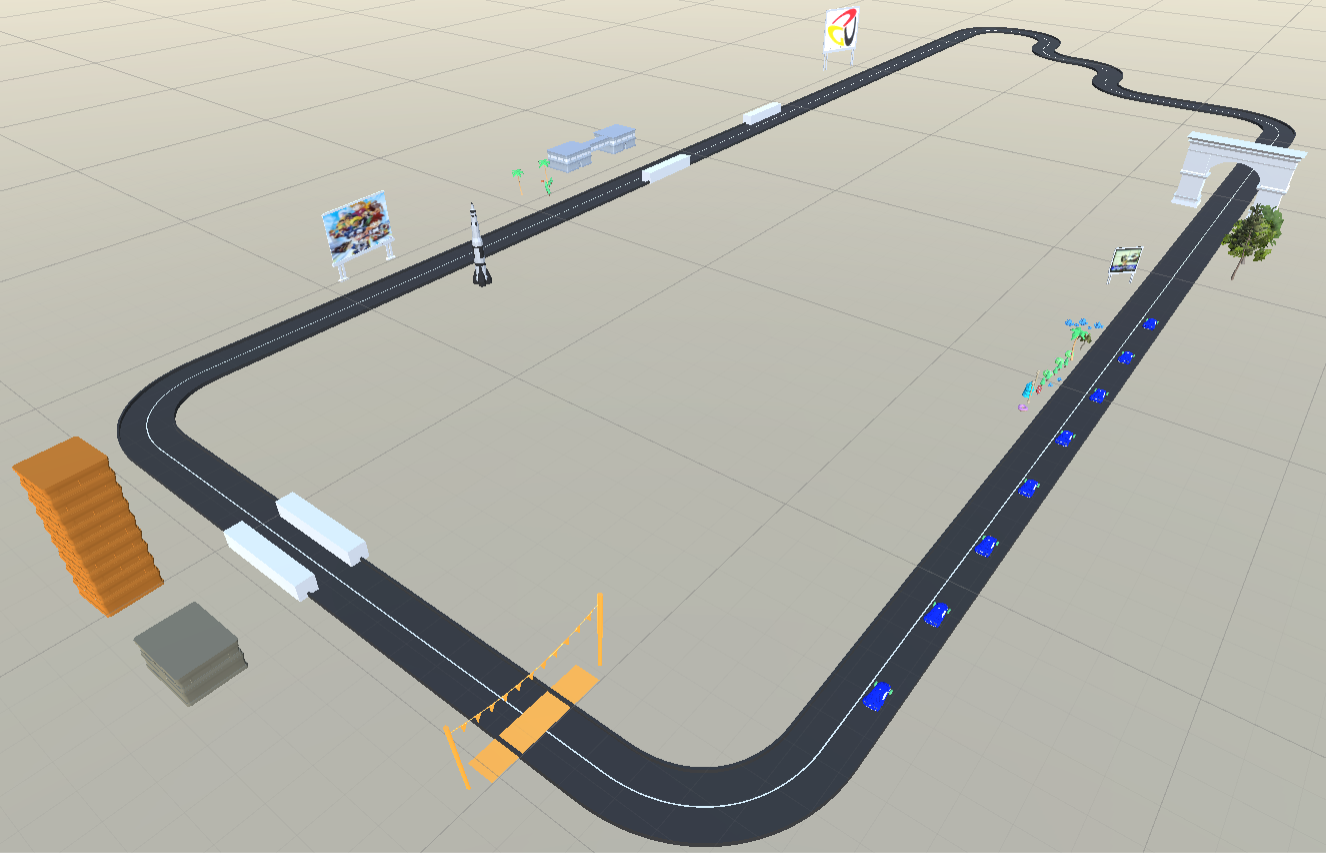
\includegraphics[scale=0.3]{Figures/EnvTest4.PNG}
    \caption{Test}
    \label{fig:my_label}
\end{figure}

Also there are two test scenarios to be tested to validate scalability of the length of the platoon and decentralization of agents. First scenario
\end{comment}



\subsection{Evaluation metrics}
 SDCP performance will be evaluated by Root Mean Square Error (RMSE), Standard Deviation (Std), maximum gap, and stalled gap values for the gap error between the vehicles and the number of crashes which is one of the main perspectives of safe driving validation.
The test track is designed to be as complex as the training track but with new scenarios like passing through a narrow way between two obstacles as shown in Figure 9 and this complexity is to simulate real hard maneuvers for the human drivers themselves. Agents have no prior knowledge of the test track design or obstacle locations and their objective is to keep driving in platoon formation and respect its rules as much as possible while being able to handle driving safely and solely if needed. Table II shows the driving distance for each test case experiment.\\
Five test case scenarios are conducted to test the performance of SDCP and each test case is to validate one of the core concepts of the developed platoon. The first test case is to test scalability by increasing the number of vehicles in the platoon from three vehicles, as in the training process, to eight vehicles. The second test is for measuring the cooperation between vehicles in dealing with aggressive maneuvers from the leader vehicle. The third test is for validating decentralization where followers are subjected to drive without the leader, and this simulates a real-life scenario like if the leader vehicle of the platoon has a malfunction and the platoon should continue without the leader till reaching the desired destination for time-saving. The fourth test is for the whole platoon, SDCP, driving on the testing track. The fifth test case is for measuring the impact of the developed SDCP on decreasing traffic congestion.

%Driving distance in each scenario
\begin{table}
\centering
\caption{Driving distance for each test case} 
\resizebox{8.5cm}{!}{
\renewcommand{\arraystretch}{2}
\begin{tabular} {|c||c|c|c|c|c|c|} 
 \hline
 \textbf{Test Case no.} & \textbf{Test Case 1} & \textbf{Test Case 2} & \textbf{Test Case 3} & \textbf{Test Case 4} & \textbf{Test Case 5}\\
 \hline
 Track length & 750 m & 750 m & 750 m & 1000 m & 1000 m\\
 \hline
\end{tabular} }
\end{table}

\begin{comment}
In testing, the length of the platoon is increased to eight vehicles to, and to validate decentralization followers are subjected to drive without the leader, and this simulates real-life scenario like if the leader vehicle of the platoon has a malfunction and the platoon should continue without the leader till reaching the desired destination for time-saving.


\begin{table}
\centering
\caption{Driving distance and number of Accidents for each test case} 
\resizebox{8.5cm}{!}{
\renewcommand{\arraystretch}{1.5}
\begin{tabular} {|c||c|c|c|c|c|c|} 
 \hline
 \textbf{Test Case no.} & \textbf{Test Case 1} & \textbf{Test Case 2} & \textbf{Test Case 3} & \textbf{Test Case 4} & \textbf{Test Case 5 (V2V on)} & \textbf{Test Case 5 (V2V off)}\\
 \hline
 Track length & 750 m & 750 m & 750 m & 1000 m & 1000 m & 1000 m\\
 \hline
 Accidents & 0 & 0 & 0 & 0 & 0 & 1\\
\hline
\end{tabular} }
\end{table}
\end{comment}


\begin{figure}
    \centering
    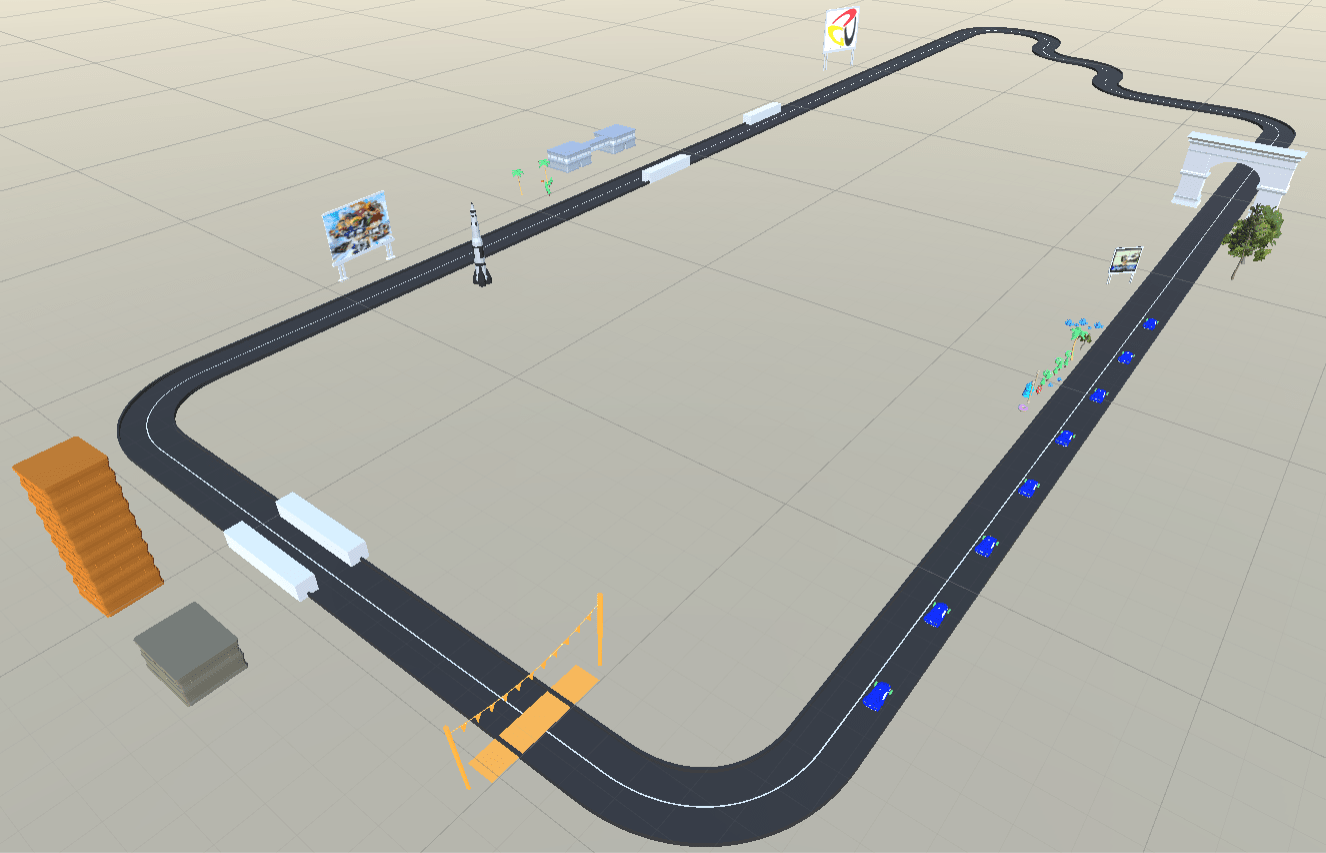
\includegraphics[scale=0.3]{Figures/EnvTest4-min.PNG}
    \caption{Urban Testing Track}
    \label{fig:my_label}
\end{figure}


